\documentclass[tikz,border=3.14mm]{standalone}
\begin{document}
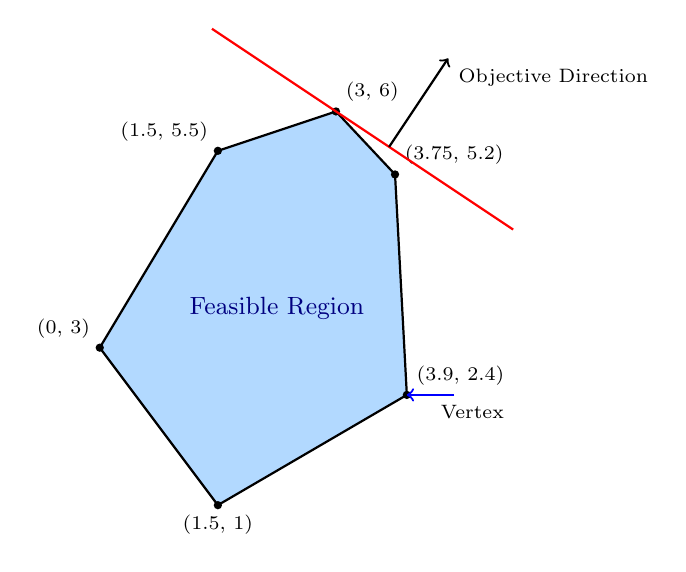
\begin{tikzpicture}

    % Define direction d as a variable
    \pgfmathsetmacro{\dx}{2.25} % Adjusted for 1.5x scaling
    \pgfmathsetmacro{\dy}{-1.5}

    % Compute perpendicular direction to d
    \pgfmathsetmacro{\dperpx}{-\dy}
    \pgfmathsetmacro{\dperpy}{\dx}

    % Define the polygon fill with scaled coordinates
    \fill[blue!50!cyan,opacity=0.3] 
        (0,3) -- (1.5,5.5) -- (3,6) -- (3.75,5.2) -- (3.9,2.4) -- (1.5,1) -- cycle;

    % Draw the polygon outline
    \draw[thick] 
        (0,3) -- (1.5,5.5) -- (3,6) -- (3.75,5.2) -- (3.9,2.4) -- (1.5,1) -- cycle;

    % Draw the nodes (points) and label them with coordinates
    \foreach \x/\y in {  3/6, 3.75/5.2, 3.9/2.4} {
        \fill[black] (\x,\y) circle (1.5pt);
        \node[font=\scriptsize, above right] at (\x,\y) {(\x, \y)};
    }
        \foreach \x/\y in {0/3, 1.5/5.5} {
        \fill[black] (\x,\y) circle (1.5pt);
        \node[font=\scriptsize, above left] at (\x,\y) {(\x, \y)};
    }
          \foreach \x/\y in {1.5/1} {
        \fill[black] (\x,\y) circle (1.5pt);
        \node[font=\scriptsize, below] at (\x,\y) {(\x, \y)};
    }

    % Define the red line through (3,6) in direction d
    \draw[red, thick] 
        ({3 + \dx}, {6 + \dy}) -- ({3 - 0.7*\dx}, {6 - 0.7*\dy});

    % Add a perpendicular arrow at (3,6)
    \draw[->, thick] 
        ({3 + 0.3*\dx}, {6 + 0.3*\dy}) -- 
        ({3 + 0.3*\dx + 0.5*\dperpx}, {6 + 0.3*\dy + 0.5*\dperpy})
        node[below right, font=\scriptsize] {Objective Direction};

    % Add a label for the feasible region
    \node[blue!50!black, font=\small] at (2.25, 3.5) {Feasible Region};

    % Add an arrow pointing to a vertex and label the vertex
    \draw[->, thick, blue] (4.5, 2.4) -- (3.9,2.4) 
        node[midway, below right, black, font=\scriptsize] {Vertex};

\end{tikzpicture}
\end{document}
